\documentclass[9pt,a4paper]{article}
\usepackage[utf8]{inputenc}
\usepackage[margin=1.15cm,footskip=0pt,headsep=0pt]{geometry}
\usepackage{mathpazo} % Classic Academic Serif Font (Palatino)
\usepackage[scaled=0.95]{helvet}
\usepackage{amsmath,amssymb}
\usepackage{xcolor}
\usepackage{tabularx}
\usepackage{booktabs}
\usepackage{enumitem}
\usepackage{tikz}
\usetikzlibrary{arrows.meta,positioning,shapes.geometric}
\usepackage{hyperref}

% STRICTLY NO RUNNING HEADERS, NO FOOTERS
\pagestyle{empty}
\thispagestyle{empty}

\raggedbottom
\setlength{\parindent}{0pt}
\setlength{\parskip}{2.8pt}

% Selective Semantic Highlights (Rare & Purposeful)
\definecolor{hlgray}{HTML}{E2E8F0}
\definecolor{hlyellow}{HTML}{FEF08A}
\definecolor{hlred}{HTML}{FEE2E2}
\definecolor{darkred}{HTML}{991B1B}
\definecolor{navy}{HTML}{0A2540}

\newcommand{\hlg}[1]{\colorbox{hlgray}{\strut #1}}
\newcommand{\hly}[1]{\colorbox{hlyellow}{\strut #1}}
\newcommand{\hlr}[1]{\colorbox{hlred}{\strut\color{darkred}#1}}

\hypersetup{
    colorlinks=true,
    linkcolor=navy,
    citecolor=navy,
    urlcolor=navy
}

\setlist[itemize]{leftmargin=1.1em, itemsep=1.2pt, topsep=1pt, parsep=0pt}
\setlist[enumerate]{leftmargin=1.1em, itemsep=1.2pt, topsep=1pt, parsep=0pt}

\begin{document}

% =========================================================================
% PAGE 1: SCOPE, MALIGNANT TRANSFORMATION & DIAGNOSTIC/SURVEILLANCE MANDATES
% =========================================================================

\begin{center}
{\Large\bfseries Evidence-Based Clinical Practice Guideline: Oral Leukoplakia}\\[2pt]
{\small\itshape Risk Stratification, Diagnostic Protocols, Interventional Matrix \& Refractory Escalation}
\end{center}
\vspace{-4pt}
\hrule height 0.8pt
\vspace{4pt}

\textbf{Clinical Definition (WHO Collaborating Centre 2021):}
Oral leukoplakia is defined as \textit{``a predominantly white plaque of questionable risk having excluded other known diseases or disorders that carry no increased risk for cancer.''} Global adult pooled prevalence: \hlg{2.60\%} (95\% CI: 1.72\%--3.74\%).

\textbf{Slaughter's Field Cancerization Mandate:}
Complete surgical excision or clinical clearance \underline{does not eliminate oral cancer risk}. Genetically altered, subclinical mucosal fields (harboring 3p/9p loss and aneuploidy) persist beyond resection margins. \hly{Active clinical surveillance is mandatory and lifelong} (\href{https://pubmed.ncbi.nlm.nih.gov/27471822/}{Cochrane CD001829}).

\vspace{2pt}
{\large\bfseries 1. Malignant Transformation (MT) \& Risk Stratification}
\vspace{1pt}

Pooled meta-analytic transformation hazards synthesized from multi-center global cohorts ($\text{n}>20,000$ patients):

\vspace{1pt}
\begin{center}
\footnotesize
\renewcommand{\arraystretch}{1.12}
\begin{tabularx}{\linewidth}{>{\raggedright\arraybackslash}p{4.3cm} c c >{\raggedright\arraybackslash}X}
\toprule
\textbf{Clinical / Histopathologic Stratum} & \textbf{Pooled MT Rate} & \textbf{Annualized Hazard} & \textbf{PubMed Landmark Citation} \\
\midrule
\textbf{Global Pooled Oral Leukoplakia} & \textbf{\hlg{7.2\% -- 9.5\%}} & \textbf{1.56\% / year} & Aguirre-Urizar (2021, \href{https://pubmed.ncbi.nlm.nih.gov/33496377/}{PMID: 33496377}); Iocca (2020) \\
Homogeneous Leukoplakia & 3.0\% (1.2\%--4.9\%) & 0.4\% -- 0.8\% / year & Warnakulasuriya (2020, \href{https://pubmed.ncbi.nlm.nih.gov/32529681/}{PMID: 32529681}); Holmstrup (2006) \\
Erythroleukoplakia (Speckled) & \hly{14.5\% -- 28.7\%} & 2.9\% -- 5.4\% / year & Warnakulasuriya (2020) [RR: 4.15]; Holmstrup (2006) \\
Nodular / Verrucous Leukoplakia & 15.0\% -- 24.5\% & 2.5\% -- 4.1\% / year & Napier \& Speight (2008, \href{https://pubmed.ncbi.nlm.nih.gov/18783457/}{PMID: 18783457}); Dionne (2015) \\
\textbf{Proliferative Verrucous (PVL)} & \textbf{\hlr{49.5\% -- 65.8\%}} & \textbf{9.3\% -- 14.2\% / year} & Villa et al. (2018, \href{https://pubmed.ncbi.nlm.nih.gov/30527232/}{PMID: 30527232}); Bagan (2010) \\
\midrule
\textit{No Dysplasia (Keratosis / Acanthosis)} & 1.5\% -- 3.9\% & 0.3\% / year & Mehanna et al. (2009, \href{https://pubmed.ncbi.nlm.nih.gov/19800840/}{PMID: 19800840}); Warnakulasuriya (2015) \\
\textit{Mild Epithelial Dysplasia} & 4.8\% -- 10.3\% & 1.1\% / year & Mehanna et al. (2009 pooled meta-analysis) \\
\textit{Moderate Epithelial Dysplasia} & \hly{15.7\% -- 24.1\%} & 3.2\% / year & Kujan et al. (2006, \href{https://pubmed.ncbi.nlm.nih.gov/16960010/}{PMID: 16960010}); Mehanna et al. (2009) \\
\textit{Severe Dysplasia / CIS} & \hlr{24.1\% -- 43.5\%} & 5.8\% -- 8.5\% / year & Warnakulasuriya (2020); Rock et al. (2018, \href{https://pubmed.ncbi.nlm.nih.gov/29778738/}{PMID: 29778738}) \\
\bottomrule
\end{tabularx}
\end{center}

\vspace{-2pt}
\textbf{Multivariate Prognosticators:}
\begin{itemize}
    \item \textbf{High-Risk Subsites:} \hly{Ventral tongue, floor of mouth, and lateral tongue} exhibit $HR = 2.45$ ($p<0.001$).
    \item \textbf{Lesion Dimension:} Lesions $>200\text{ mm}^2$ ($>2\text{ cm}$) exhibit $HR = 3.20$ for malignant progression.
    \item \textbf{Non-Smoker Paradox:} Non-smoking elderly females exhibit $RR = 2.14$ ($95\%$ CI: 1.42--3.22) due to endogenous driver mutations.
    \item \textbf{Genomic Biomarkers (LoE 1b):} 3p/9p loss of heterozygosity elevates cancer hazard $8.4$-fold; combined 3p/9p/17p loss elevates hazard $33$-fold. DNA aneuploidy confers $HR = 3.65$.
\end{itemize}

\vspace{2pt}
{\large\bfseries 2. Diagnostic Protocol, Biopsy Mandates \& Surveillance Schedule}
\vspace{1pt}

\begin{itemize}
    \item \textbf{Diagnostic Standard:} Formal \underline{scalpel incisional biopsy} including adequate lamina propria depth is mandatory for white lesions persisting $>14$ days post-elimination of frictional irritants and completion of antifungal trial. Multi-site mapping biopsies are compulsory for lesions $>2\text{ cm}$ or non-homogeneous plaques (single biopsies miss advanced dysplasia in $\approx 30\%$).
    \item \textbf{Optical Diagnostic Adjuncts:} Autofluorescence (VELscope) and toluidine blue have poor specificity ($45\text{--}60\%$); they are strictly adjunctive and \underline{never replace histopathology} (WHO 2021).
    \item \textbf{Evidence-Based Surveillance Schedule:}
    \begin{itemize}
        \item \textit{Low-Risk Homogeneous (No dysplasia, $<2\text{ cm}$):} \hlg{Every 6 months} lifelong.
        \item \textit{Intermediate-Risk (Mild dysplasia or $>2\text{ cm}$):} \hlg{Every 3--4 months} for years 1--2, then every 6 months.
        \item \textit{High-Risk / Post-Resection (Moderate/Severe dysplasia, CIS):} \hlg{Every 2--3 months} for year 1, every 3--4 months for years 2--3, then every 6 months lifelong.
        \item \textit{Proliferative Verrucous Leukoplakia (PVL):} \hlr{Every 1--2 months} lifelong.
    \end{itemize}
    \item \textbf{Mandatory Biopsy Triggers:} \hly{Immediate incisional re-biopsy is required} upon: (1) emergence of erythroplakia/speckling, (2) palpable induration or verrucous texture, (3) ulceration/erosion/bleeding, (4) rapid expansion $>20\%$ in 3 months, (5) unexplained local pain/paresthesia, or (6) cervical lymphadenopathy.
\end{itemize}

\clearpage
% =========================================================================
% PAGE 2: FULL-PAGE PURE BLACK AND WHITE CLINICAL FLOWCHART (CLEAN TIKZ)
% =========================================================================

\begin{center}
{\Large\bfseries Clinical Decision Flowchart: Oral Leukoplakia}\\[2pt]
{\small\itshape Systematic Pathway: Diagnostic Triage, Histopathologic Stratification, Intervention \& Recall}
\end{center}
\vspace{-4pt}
\hrule height 0.8pt
\vspace{10pt}

\begin{center}
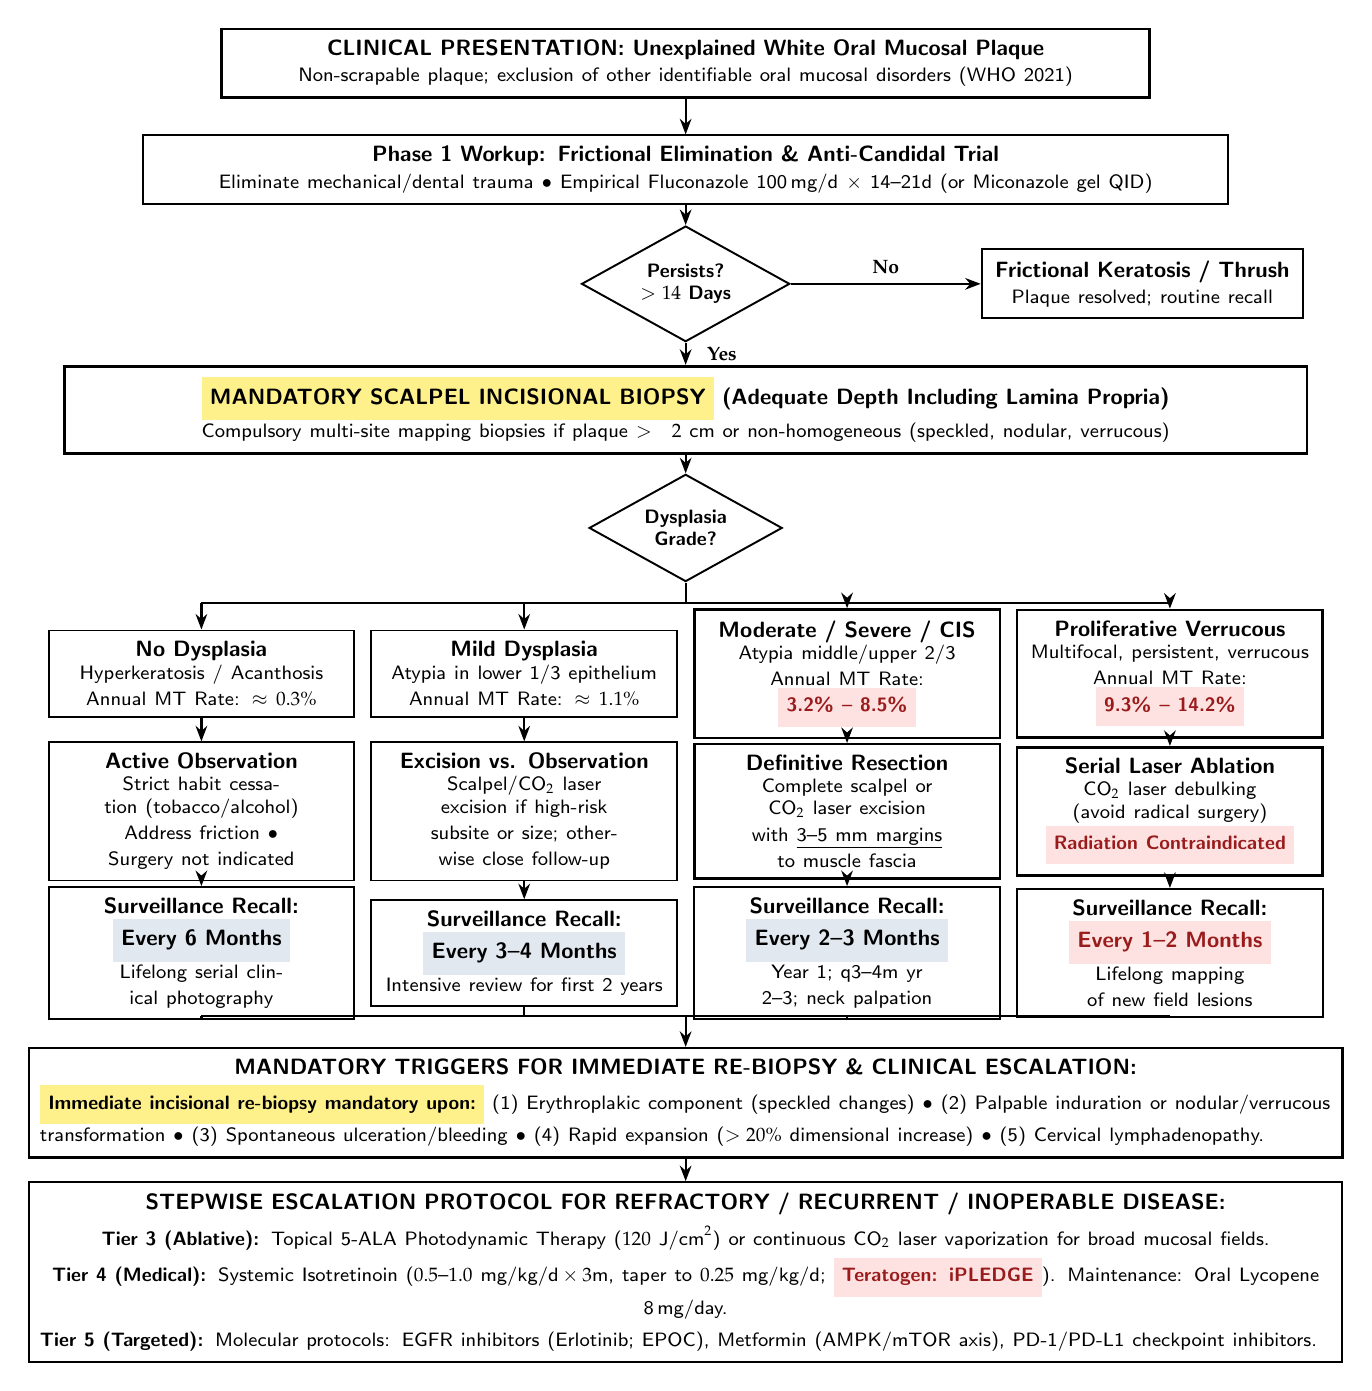
\begin{tikzpicture}[
    every node/.style={font=\sffamily\footnotesize, align=center},
    stepbox/.style={rectangle, draw=black, fill=white, line width=0.7pt, inner sep=4pt},
    decision/.style={diamond, aspect=1.8, draw=black, fill=white, line width=0.7pt, inner sep=3pt, font=\sffamily\scriptsize\bfseries},
    arrow/.style={-{Stealth[scale=0.85]}, thick, black}
]

% 1. Initial Presentation
\node (n1) [stepbox, line width=1.0pt, text width=11.5cm] at (0, 0) {
    \textbf{CLINICAL PRESENTATION: Unexplained White Oral Mucosal Plaque}\\
    \scriptsize Non-scrapable plaque; exclusion of other identifiable oral mucosal disorders (WHO 2021)
};

% 2. Screening & Elimination
\node (n2) [stepbox, text width=13.5cm] at (0, -1.35) {
    \textbf{Phase 1 Workup: Frictional Elimination \& Anti-Candidal Trial}\\
    \scriptsize Eliminate mechanical/dental trauma $\bullet$ Empirical Fluconazole 100\,mg/d $\times$ 14--21d (or Miconazole gel QID)
};

% 3. Persistence Decision
\node (d1) [decision] at (0, -2.8) {\textbf{Persists?}\\\scriptsize $>14$ Days};
\node (r_benign) [stepbox, text width=3.8cm] at (5.8, -2.8) {
    \textbf{Frictional Keratosis / Thrush}\\
    \scriptsize Plaque resolved; routine recall
};

% 4. Mandatory Biopsy
\node (n3) [stepbox, line width=1.0pt, text width=15.5cm] at (0, -4.4) {
    \textbf{\hly{MANDATORY SCALPEL INCISIONAL BIOPSY} (Adequate Depth Including Lamina Propria)}\\
    \scriptsize Compulsory multi-site mapping biopsies if plaque $>2\text{ cm}$ or non-homogeneous (speckled, nodular, verrucous)
};

% 5. Histopathology Decision
\node (d2) [decision] at (0, -5.9) {\textbf{Dysplasia}\\\scriptsize Grade?};

% 6. Histopathology 4 Columns: Centers at -6.15, -2.05, 2.05, 6.15 (Width 3.8cm, Text width 3.6cm)
\node (h1) [stepbox, text width=3.6cm] at (-6.15, -7.75) {
    \textbf{No Dysplasia}\\
    \scriptsize Hyperkeratosis / Acanthosis\\Annual MT Rate: $\approx 0.3\%$
};
\node (h2) [stepbox, text width=3.6cm] at (-2.05, -7.75) {
    \textbf{Mild Dysplasia}\\
    \scriptsize Atypia in lower 1/3 epithelium\\Annual MT Rate: $\approx 1.1\%$
};
\node (h3) [stepbox, line width=0.9pt, text width=3.6cm] at (2.05, -7.75) {
    \textbf{Moderate / Severe / CIS}\\
    \scriptsize Atypia middle/upper 2/3\\Annual MT Rate: \hlr{\textbf{3.2\% -- 8.5\%}}
};
\node (h4) [stepbox, line width=1.0pt, text width=3.6cm] at (6.15, -7.75) {
    \textbf{Proliferative Verrucous}\\
    \scriptsize Multifocal, persistent, verrucous\\Annual MT Rate: \hlr{\textbf{9.3\% -- 14.2\%}}
};

% 7. Interventions (3 Lines per column for uniform height)
\node (i1) [stepbox, text width=3.6cm] at (-6.15, -9.5) {
    \textbf{Active Observation}\\
    \scriptsize Strict habit cessation (tobacco/alcohol)\\Address friction $\bullet$ Surgery not indicated
};
\node (i2) [stepbox, text width=3.6cm] at (-2.05, -9.5) {
    \textbf{Excision vs. Observation}\\
    \scriptsize Scalpel/$\text{CO}_2$ laser excision if high-risk\\subsite or size; otherwise close follow-up
};
\node (i3) [stepbox, line width=0.9pt, text width=3.6cm] at (2.05, -9.5) {
    \textbf{Definitive Resection}\\
    \scriptsize Complete scalpel or $\text{CO}_2$ laser excision\\with \underline{3--5 mm margins} to muscle fascia
};
\node (i4) [stepbox, line width=1.0pt, text width=3.6cm] at (6.15, -9.5) {
    \textbf{Serial Laser Ablation}\\
    \scriptsize $\text{CO}_2$ laser debulking (avoid radical surgery)\\\hlr{\textbf{Radiation Contraindicated}}
};

% 8. Recall Schedules (3 Lines per column for uniform height)
\node (s1) [stepbox, text width=3.6cm] at (-6.15, -11.3) {
    \textbf{Surveillance Recall:}\\[1pt]
    \hlg{\textbf{Every 6 Months}}\\
    \scriptsize Lifelong serial clinical photography
};
\node (s2) [stepbox, text width=3.6cm] at (-2.05, -11.3) {
    \textbf{Surveillance Recall:}\\[1pt]
    \hlg{\textbf{Every 3--4 Months}}\\
    \scriptsize Intensive review for first 2 years
};
\node (s3) [stepbox, text width=3.6cm] at (2.05, -11.3) {
    \textbf{Surveillance Recall:}\\[1pt]
    \hlg{\textbf{Every 2--3 Months}}\\
    \scriptsize Year 1; q3--4m yr 2--3; neck palpation
};
\node (s4) [stepbox, text width=3.6cm] at (6.15, -11.3) {
    \textbf{Surveillance Recall:}\\[1pt]
    \hlr{\textbf{Every 1--2 Months}}\\
    \scriptsize Lifelong mapping of new field lesions
};

% 9. Trigger Box
\node (trigger) [stepbox, line width=0.9pt, text width=16.4cm, align=left] at (0, -13.2) {
    \centering\textbf{MANDATORY TRIGGERS FOR IMMEDIATE RE-BIOPSY \& CLINICAL ESCALATION:}\\[3pt]
    \scriptsize \hly{\textbf{Immediate incisional re-biopsy mandatory upon:}} (1) Erythroplakic component (speckled changes) $\bullet$ (2) Palpable induration or nodular/verrucous transformation $\bullet$ (3) Spontaneous ulceration/bleeding $\bullet$ (4) Rapid expansion ($>20\%$ dimensional increase) $\bullet$ (5) Cervical lymphadenopathy.
};

% 10. Refractory Box
\node (refract) [stepbox, text width=16.4cm, align=left] at (0, -15.35) {
    \centering\textbf{STEPWISE ESCALATION PROTOCOL FOR REFRACTORY / RECURRENT / INOPERABLE DISEASE:}\\[3pt]
    \scriptsize \textbf{Tier 3 (Ablative):} Topical 5-ALA Photodynamic Therapy ($120\text{ J/cm}^2$) or continuous $\text{CO}_2$ laser vaporization for broad mucosal fields.\\[2pt]
    \textbf{Tier 4 (Medical):} Systemic Isotretinoin ($0.5\text{--}1.0\text{ mg/kg/d}\times 3\text{m}$, taper to $0.25\text{ mg/kg/d}$; \hlr{\textbf{Teratogen: iPLEDGE}}). Maintenance: Oral Lycopene 8\,mg/day.\\[2pt]
    \textbf{Tier 5 (Targeted):} Molecular protocols: EGFR inhibitors (Erlotinib; EPOC), Metformin (AMPK/mTOR axis), PD-1/PD-L1 checkpoint inhibitors.
};

% Connections
\draw [arrow] (n1) -- (n2);
\draw [arrow] (n2) -- (d1);
\draw [arrow] (d1.east) -- node[above, font=\scriptsize\bfseries] {No} (r_benign.west);
\draw [arrow] (d1.south) -- node[right=4pt, font=\scriptsize\bfseries] {Yes} (n3.north);
\draw [arrow] (n3.south) -- (d2.north);

% Clean Bus-Bar from Decision 2 to 4 Histology columns (Completely untangled!)
\draw [thick, black] (d2.south) -- (0, -6.85);
\draw [thick, black] (-6.15, -6.85) -- (6.15, -6.85);
\draw [arrow] (-6.15, -6.85) -- (h1.north);
\draw [arrow] (-2.05, -6.85) -- (h2.north);
\draw [arrow] (2.05, -6.85) -- (h3.north);
\draw [arrow] (6.15, -6.85) -- (h4.north);

% Column Downward Arrows
\draw [arrow] (h1) -- (i1);
\draw [arrow] (h2) -- (i2);
\draw [arrow] (h3) -- (i3);
\draw [arrow] (h4) -- (i4);

\draw [arrow] (i1) -- (s1);
\draw [arrow] (i2) -- (s2);
\draw [arrow] (i3) -- (s3);
\draw [arrow] (i4) -- (s4);

% Collector Bus into Trigger Box
\draw [thick, black] (s1.south) -- (-6.15, -12.1);
\draw [thick, black] (s2.south) -- (-2.05, -12.1);
\draw [thick, black] (s3.south) -- (2.05, -12.1);
\draw [thick, black] (s4.south) -- (6.15, -12.1);
\draw [thick, black] (-6.15, -12.1) -- (6.15, -12.1);
\draw [arrow] (0, -12.1) -- (trigger.north);

\draw [arrow] (trigger.south) -- (refract.north);

\end{tikzpicture}
\end{center}

\clearpage
% =========================================================================
% PAGE 3: EVIDENCE-BASED CLINICAL GUIDELINE MASTER MATRIX (EXACT 1 PAGE)
% =========================================================================

\begin{center}
{\Large\bfseries Evidence-Based Clinical Guideline Master Matrix}\\[2pt]
{\small Operationalized Recommendations Indexed to GRADE Framework and Oxford CEBM (2011) Criteria}
\end{center}
\vspace{-4pt}
\hrule height 0.8pt
\vspace{5pt}

\footnotesize
\setlength{\tabcolsep}{3.5pt}
\renewcommand{\arraystretch}{1.10}
\begin{tabularx}{\linewidth}{>{\raggedright\arraybackslash}p{2.8cm} >{\raggedright\arraybackslash}p{3.8cm} >{\raggedright\arraybackslash}p{2.0cm} >{\raggedright\arraybackslash}p{5.1cm} >{\raggedright\arraybackslash}X}
\toprule
\textbf{Clinical Subtype} & \textbf{Recommended Intervention} & \textbf{GRADE \& LoE} & \textbf{Monitoring, Tapering \& Safety Contraindications} & \textbf{PubMed Citation} \\
\midrule
\textbf{1. Low-Risk Homogeneous}\newline\scriptsize ($<2\text{ cm}$, buccal mucosa, non-dysplastic) &
Conservative surveillance; strict tobacco and alcohol cessation; eliminate dental friction. &
GRADE A [Strong]\newline LoE 1a / 1b &
Review photography \hlg{every 6 months}. Routine surgical excision is not recommended (surgical morbidity exceeds risk; no MT reduction). &
Warnakulasuriya (2020);\newline Lodi (2016, Cochrane);\newline \href{https://pubmed.ncbi.nlm.nih.gov/32529681/}{\textbf{PMID: 32529681}} \\
\midrule
\textbf{2. Candidal Leukoplakia}\newline\scriptsize (Chronic hyperplastic candidiasis; PAS+ hyphae) &
Fluconazole 100\,mg PO QD $\times$ 14--28 days.\newline\textit{Topical Alt:} Miconazole oral gel 24\,mg/g, 2.5\,mL QID $\times$ 21 days. &
GRADE A [Strong]\newline LoE 1a / 1b &
Re-evaluate at 14 and 28 days. \underline{Mandatory re-biopsy} if plaque persists. Monitor LFTs if systemic therapy $>14$ days. CYP3A4 interactions. &
Sitheeamorn (2022);\newline Williams (2014, Oral Dis);\newline \href{https://pubmed.ncbi.nlm.nih.gov/24750244/}{\textbf{PMID: 24750244}} \\
\midrule
\textbf{3. Moderate / Severe Dysplasia; High-Risk Subsite} &
Definitive cold scalpel or $\text{CO}_2$ laser excision (10.6\,$\mu$m, 5--10\,W) with \underline{3--5\,mm clear margins} to muscular fascia. &
GRADE A [Strong]\newline LoE 1a / 1b &
Histologic margin analysis. Dysplastic cut margins mandate staged re-excision or intensified 8-week surveillance. Recall \hlg{q2--3m} in year 1. &
WHO Guidelines (2021);\newline Mehanna (2009, Lancet);\newline \href{https://pubmed.ncbi.nlm.nih.gov/19800840/}{\textbf{PMID: 19800840}} \\
\midrule
\textbf{4. Erythroleukoplakia}\newline\scriptsize (Speckled leukoplakia; high malignant hazard) &
Complete scalpel or $\text{CO}_2$ laser excision. Multi-site mapping biopsies if $>3\text{ cm}$ followed by staged excision. &
GRADE A [Strong]\newline LoE 2a / 2b &
Intensive surveillance \hlg{every 2 months} for first 12 months. Frozen sections if micro-invasion suspected. Bimanual neck examination. &
Warnakulasuriya (2020);\newline Holmstrup (2006, Oral Onc);\newline \href{https://pubmed.ncbi.nlm.nih.gov/16406797/}{\textbf{PMID: 16406797}} \\
\midrule
\textbf{5. Proliferative Verrucous (PVL)} &
Serial conservative $\text{CO}_2$ laser ablation for thick verrucous plaques. Avoid extensive disfiguring resections (recurrence $>85\%$). &
GRADE B [Moderate]\newline LoE 2a / 2b &
Ultra-intensive recall \hlr{every 1--2 months} lifelong. \hlr{\textbf{Radiation is strictly contraindicated}} (triggers rapid anaplastic dedifferentiation). &
Villa et al. (2018, Oral Onc);\newline Bagan (2010, Med Oral);\newline \href{https://pubmed.ncbi.nlm.nih.gov/30527232/}{\textbf{PMID: 30527232}} \\
\midrule
\textbf{6. Inoperable / Refractory Leukoplakia} &
Isotretinoin (13-\textit{cis}-retinoic acid): 0.5--1.0\,mg/kg/day PO BID $\times$ 3 months. Taper to 0.25\,mg/kg/day for 6--9 months. &
GRADE B [Moderate]\newline LoE 1a / 1b &
\hlr{\textbf{Category X (Teratogen)}}: negative monthly $\beta$-hCG and dual contraception (iPLEDGE). Monitor fasting lipid panel and LFTs at baseline, wk 2, 4, then monthly. &
Hong (1986, NEJM);\newline Lippman (1993, NEJM);\newline \href{https://pubmed.ncbi.nlm.nih.gov/8464432/}{\textbf{PMID: 8464432}} \\
\midrule
\textbf{7. Superficial Recurrent Dysplastic Plaques} &
Photodynamic Therapy (PDT): Topical 5-ALA 20\% gel applied 3--4h; diode laser 630--635\,nm ($100\text{--}150\text{ J/cm}^2$). Repeat q2--4w $\times$ 1--4 cycles. &
GRADE B [Moderate]\newline LoE 2a / 2b &
Assess mucosal re-epithelialization at 2 weeks. Post-treatment necrosis and edema expected. Strict light avoidance $\times$ 48h to prevent cutaneous photosensitivity. &
Sieron (2003, Photodiag);\newline Yu (2009, Oral Oncol);\newline \href{https://pubmed.ncbi.nlm.nih.gov/19443260/}{\textbf{PMID: 19443260}} \\
\midrule
\textbf{8. Chemoprevention / Maintenance} &
Oral Lycopene 8\,mg daily (divided 4\,mg BID) $\times$ 3 months. Modulates antioxidant response and IGFBP-3 expression. &
GRADE C [Conditional]\newline LoE 2a / 2b &
Measure plaque dimensions at 4, 8, 12 weeks. Minimal toxicity (mild transient diarrhea). Completely devoid of teratogenic or hepatotoxic liabilities. &
Nagao (2015, Cancer Prev);\newline Zakrzewska (2005);\newline \href{https://pubmed.ncbi.nlm.nih.gov/25770020/}{\textbf{PMID: 25770020}} \\
\bottomrule
\end{tabularx}

\vspace{5pt}
\textbf{Methodological Directive on Surgical Margins:} Mild dysplasia at excision margins does not require mandatory re-resection if strict 3-month clinical surveillance is enforced. Moderate/severe dysplasia or carcinoma \textit{in situ} at margins increases local recurrence $2.8$-fold, mandating staged re-excision or intensified 8-week surveillance (\href{https://pubmed.ncbi.nlm.nih.gov/19800840/}{Mehanna 2009}).

\clearpage
% =========================================================================
% PAGE 4: REFRACTORY ALGORITHM & VERIFIED PUBMED SOURCES
% =========================================================================

\begin{center}
{\Large\bfseries Refractory Case Algorithm \& Stepwise Escalation}\\[2pt]
{\small Step-Up Protocols for Persistent, Recurrent, or Broad-Field Dysplastic Disease}
\end{center}
\vspace{-4pt}
\hrule height 0.8pt
\vspace{5pt}

\begin{itemize}
    \item \textbf{Tier 1: Baseline Elimination \& Diagnostic Verification:} Complete cessation of tobacco, alcohol, and areca nut. Smooth sharp restorations. Antifungal trial (Fluconazole 100\,mg/day $\times$ 21 days). Persistent lesions undergo repeat mapping incisional biopsies.
    \item \textbf{Tier 2: Primary Surgical / Laser Resection:} Cold knife or $\text{CO}_2$ laser excision with \underline{3--5\,mm clinical margins} to muscular fascia for moderate/severe dysplasia. Positive dysplastic margins mandate re-excision or intensified 8-week surveillance.
    \item \textbf{Tier 3: Minimally Invasive Ablative Therapies:} Indicated for broad, multifocal, or anatomically restricted fields (ventral tongue, soft palate) where deep surgical resection would cause severe speech/swallowing disability. Modalities: Topical 5-ALA Photodynamic Therapy (PDT; 630\,nm, $120\text{ J/cm}^2$) or continuous-wave $\text{CO}_2$ laser vaporization.
    \item \textbf{Tier 4: Systemic Medical Pharmacotherapy:} Indicated for extensive, inoperable, or rapidly recurrent dysplastic plaques. Induction: Isotretinoin (0.5--1.0\,mg/kg/day $\times$ 3 months), tapering to maintenance (0.25\,mg/kg/day) or rotational maintenance with oral Lycopene (8\,mg/day) to mitigate the $>50\%$ relapse rate after retinoid cessation. Mandatory iPLEDGE teratogenicity protocol.
    \item \textbf{Tier 5: Investigational Targeted Biologics \& Clinical Trials:} Enrollment in controlled trials: EGFR tyrosine kinase inhibitors (Erlotinib; EPOC trial, \href{https://pubmed.ncbi.nlm.nih.gov/27091708/}{PMID: 27091708}), Metformin (AMPK/mTOR axis inhibition, 500--1000\,mg BID), or PD-1/PD-L1 checkpoint inhibitors (Nivolumab/Pembrolizumab) for high-risk refractory fields with immune infiltrates.
\end{itemize}

\vspace{5pt}
{\large\bfseries Authoritative Bibliographic References (PubMed Landmark Sources)}
\vspace{2pt}

\small
\begin{enumerate}
    \item \textbf{Warnakulasuriya S, Kujan O, Aguirre-Urizar JM, et al.} Oral potentially malignant disorders: A consensus report from an international seminar for the WHO Collaborating Centre for Oral Cancer. \textit{Oral Dis}. 2021;27(8):1865--1880. \href{https://pubmed.ncbi.nlm.nih.gov/32529681/}{\textbf{PMID: 32529681}}.
    \item \textbf{Aguirre-Urizar JM, Lafuente-Ibáñez de Mendoza I, Warnakulasuriya S.} Malignant transformation of oral leukoplakia: Systematic review and meta-analysis of the last 5 years. \textit{Oral Dis}. 2021;27(8):1881--1895. \href{https://pubmed.ncbi.nlm.nih.gov/33496377/}{\textbf{PMID: 33496377}}.
    \item \textbf{Iocca O, Sollecito TP, Alawi F, et al.} Potentially malignant disorders of the oral cavity and oral dysplasia: A systematic review and meta-analysis of malignant transformation rate. \textit{Oral Oncol}. 2020;99:104439. \href{https://pubmed.ncbi.nlm.nih.gov/31585721/}{\textbf{PMID: 31585721}}.
    \item \textbf{Lodi G, Franchini R, Warnakulasuriya S, et al.} Interventions for treating oral leukoplakia to prevent oral cancer. \textit{Cochrane Database Syst Rev}. 2016;7(7):CD001829. \href{https://pubmed.ncbi.nlm.nih.gov/27471822/}{\textbf{PMID: 27471822}}.
    \item \textbf{Villa A, Menon RS, Kerr AR, et al.} Proliferative verrucous leukoplakia: A systematic review and meta-analysis. \textit{Oral Oncol}. 2018;87:159--166. \href{https://pubmed.ncbi.nlm.nih.gov/30527232/}{\textbf{PMID: 30527232}}.
    \item \textbf{Mehanna HM, Rattay T, Smith J, McConkey CC.} Treatment and follow-up of oral dysplasia - a systematic review and meta-analysis. \textit{Head Neck}. 2009;31(12):1600--1609. \href{https://pubmed.ncbi.nlm.nih.gov/19800840/}{\textbf{PMID: 19800840}}.
    \item \textbf{Papadimitrakopoulou VA, Lee JJ, William WN Jr, et al.} Randomized trial of erlotinib versus observation in patients with high-risk premalignant oral lesions (EPOC). \textit{J Clin Oncol}. 2016;34(17):2025--2032. \href{https://pubmed.ncbi.nlm.nih.gov/27091708/}{\textbf{PMID: 27091708}}.
    \item \textbf{Lippman SM, Batsakis JG, Toth BB, et al.} Comparison of low-dose isotretinoin with beta carotene to prevent second primary tumors in patients treated for squamous cell carcinoma of the head and neck. \textit{N Engl J Med}. 1993;328(1):15--20. \href{https://pubmed.ncbi.nlm.nih.gov/8464432/}{\textbf{PMID: 8464432}}.
    \item \textbf{Nagao T, Warnakulasuriya S, Nakamura T, et al.} Chemoprevention of oral leukoplakia with lycopene: A randomized, double-blind, placebo-controlled clinical trial. \textit{Cancer Prev Res}. 2015;8(8):749--758. \href{https://pubmed.ncbi.nlm.nih.gov/25770020/}{\textbf{PMID: 25770020}}.
    \item \textbf{Holmstrup P, Vedtofte P, Reibel J, Stoltze K.} Long-term adult human oral leukoplakia follow-up: No evidence for regression of dysplasia or decrease of malignant transformation after surgical excision. \textit{Oral Oncol}. 2006;42(5):461--466. \href{https://pubmed.ncbi.nlm.nih.gov/16406797/}{\textbf{PMID: 16406797}}.
\end{enumerate}

\vspace{5pt}
\hrule height 0.6pt\vspace{3pt}
\footnotesize\textbf{Clinical Audit Benchmarks:} (1) Scalpel biopsy for persistent white lesions ($>14$ days). (2) Multi-site mapping for plaques $>2\text{ cm}$ or non-homogeneous lesions. (3) Documented Field Cancerization counseling prior to intervention. (4) iPLEDGE compliance for systemic retinoids. Quadrennial review: 2030. COI: None.

\end{document}
